%%%%%%%%%%%%%%%%%%%%%%%%%%%%%%%%%%%%%%%%%
% Short Sectioned Assignment
% LaTeX Template
% Version 1.0 (5/5/12)
%
% This template has been downloaded from:
% http://www.LaTeXTemplates.com
%
% Original author:
% Frits Wenneker (http://www.howtotex.com)
%
% License:
% CC BY-NC-SA 3.0 (http://creativecommons.org/licenses/by-nc-sa/3.0/)
%
%%%%%%%%%%%%%%%%%%%%%%%%%%%%%%%%%%%%%%%%%

%----------------------------------------------------------------------------------------
%	PACKAGES AND OTHER DOCUMENT CONFIGURATIONS
%----------------------------------------------------------------------------------------

\documentclass[paper=a4, fontsize=11pt]{scrartcl} % A4 paper and 11pt font size

\usepackage[T1]{fontenc} % Use 8-bit encoding that has 256 glyphs
%\usepackage{fourier} % Use the Adobe Utopia font for the document - comment this line to return to the LaTeX default
\usepackage[english]{babel} % English language/hyphenation
\usepackage{amsmath,amsfonts,amsthm} % Math packages
\usepackage{hyperref} %HTML package
\usepackage{pgfplots} %Makes plots in LaTeX
\usepackage{tikz} %Also tikz?
\usepgfplotslibrary{fillbetween}%Let's me fill between named plots


\usepackage{sectsty} % Allows customizing section commands
\allsectionsfont{ \normalfont\scshape} % Make all sections the default font and small caps


\renewcommand{\thesubsection}{\alph{subsection}} %Make subsections start with letters

\usepackage{fancyhdr} % Custom headers and footers
\pagestyle{fancyplain} % Makes all pages in the document conform to the custom headers and footers
\fancyhead{} % No page header - if you want one, create it in the same way as the footers below
\fancyfoot[L]{} % Empty left footer
\fancyfoot[C]{} % Empty center footer
\fancyfoot[R]{\thepage} % Page numbering for right footer
\renewcommand{\headrulewidth}{0pt} % Remove header underlines
\renewcommand{\footrulewidth}{0pt} % Remove footer underlines
\setlength{\headheight}{13.6pt} % Customize the height of the header

\numberwithin{equation}{section} % Number equations within sections (i.e. 1.1, 1.2, 2.1, 2.2 instead of 1, 2, 3, 4)
\numberwithin{figure}{section} % Number figures within sections (i.e. 1.1, 1.2, 2.1, 2.2 instead of 1, 2, 3, 4)
\numberwithin{table}{section} % Number tables within sections (i.e. 1.1, 1.2, 2.1, 2.2 instead of 1, 2, 3, 4)

\setlength\parindent{0pt} % Removes all indentation from paragraphs - comment this line for an assignment with lots of text

%----------------------------------------------------------------------------------------
%	TITLE SECTION
%----------------------------------------------------------------------------------------

\newcommand{\horrule}[1]{\rule{\linewidth}{#1}} % Create horizontal rule command with 1 argument of height

\title{	Assignment 3}

\author{Benjamin Jakubowski} % Your name

\date{\normalsize\today} % Today's date or a custom date

\begin{document}

\maketitle % Print the title

%----------------------------------------------------------------------------------------
%	PROBLEM 1
%----------------------------------------------------------------------------------------

\section{Messenger}

\subsection{Expected Manhattan Distance}

First, assuming the delivery points are uniformly spread in all of Manhattan, let $X \sim U(-1,1)$ and $Y \sim U(-6.5,6.5)$ represent the $x$ and $y$ coordinate of the delivery point. This model is depicted in the plot below:

\begin{center}
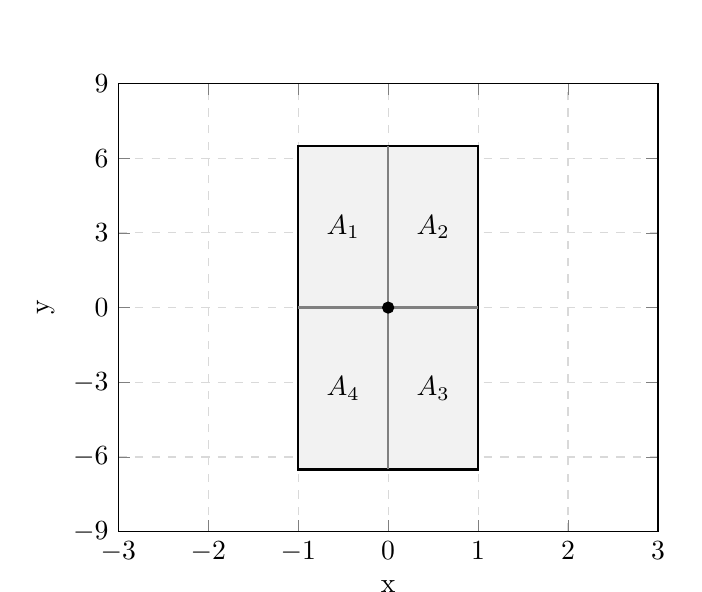
\begin{tikzpicture}
	\begin{axis}[xtick={-3,...,3}, ytick={-9,-6,...,9}, xmin=-3, xmax=3, ymin=-9, ymax=9, xlabel=x, ylabel=y, grid=major, grid style={dashed,gray!30}]
	\draw[draw=black, thick, fill =gray!10] (axis cs:-1,-6.5) rectangle (axis cs:1,6.5);
	\addplot[mark=*] coordinates {(0,0)};
	\draw[draw=gray, thick] (axis cs:0,-6.5) -- (axis cs:0,6.5);
	\draw[draw=gray, thick] (axis cs:-1,0) -- (axis cs:1,0);
	\node at (axis cs:-.5,3.25) {$A_1$};
	\node at (axis cs:.5,3.25) {$A_2$};
	\node at (axis cs:.5,-3.25) {$A_3$};
	\node at (axis cs:-.5,-3.25) {$A_4$};
	\end{axis}
\end{tikzpicture}
\end{center}

Next, note the definition of $D$ (and uniformity in the distribution of delivery points) implies:
\begin{equation*}
E[D | (x,y) \in A_i] = E[D] \textrm{  for  } i, j \in \{1,2,3,4\}
\end{equation*}
Thus, to proceed we can next limit our attention to simply $A_2$.  Then
\begin{align*}
E[D] &= E[D | (x,y) \in A_i] \\
   &= E[X + Y | (x,y) \in A_i] \\
   &= E[X | (x,y) \in A_i] + E[Y | (x,y) \in A_i]
\end{align*}
Since the joint PDF is uniform, the marginals are also uniform. Since the expected value of a $U(a,b)$ random variable is $1/2 \cdot (b - a)$,
\begin{align*}
E[D] &= E[X | (x,y) \in A_i] + E[Y | (x,y) \in A_i]\\
   &= 1/2 (1 - 0) + 1/2 (6.5 - 0) = 4.25
\end{align*}
Thus, $E[D] =4.25$.

\subsection{Bound on P(D) > 5}

Recall Markov's Inequality states, for a non-negative RV $X$:
\begin{equation*}
P(X \geq a) \leq \frac{E[X]}{a}
\end{equation*}
Thus,
\begin{equation*}
P(D \geq 5) \leq \frac{E[D]}{a} = \frac{4.25}{5} = .85
\end{equation*}

Thus, the probability a messenger has to travel more than 5 miles is less than .85.

%----------------------------------------------------------------------------------------
%	PROBLEM 2
%----------------------------------------------------------------------------------------

\section{Pasta and Rice}

\subsection{Joint PDF of $X$ and $R$}

To start, information provided by the cook implies:
\begin{align*}
P(X \geq 100 \cup R \geq 100) &= 1\\
\textrm{ and, equivalently } P(X < 100 \cap R < 100) &= 0
\end{align*}
Moreover, $P(X \leq 300) = 1$ and $P(R \leq 300) = 1$. Based on this information (and the assumption the joint pdf is constant), we can construct the joint pdf of $X$ and $R$ $f_{X,R}(x,r)$ as shown below:

\begin{center}
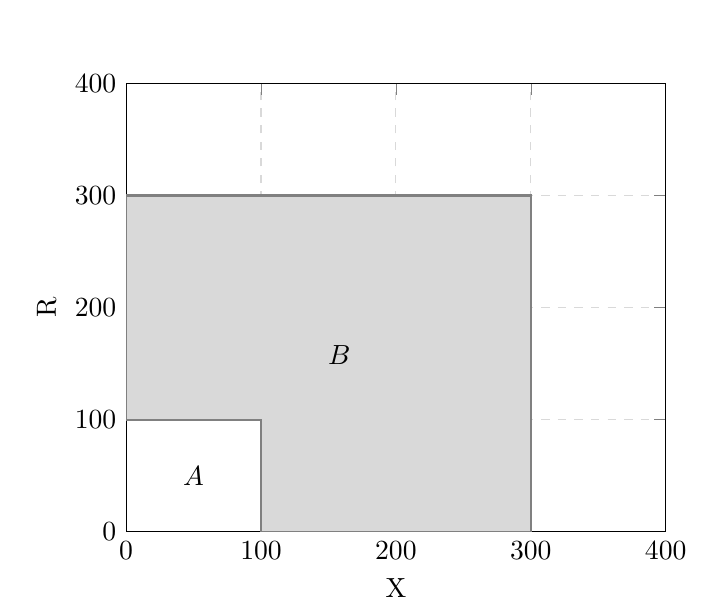
\begin{tikzpicture}
	\begin{axis}[xtick={0,100,...,400}, ytick={0,100,...,400}, xmin=0, xmax=400, ymin=0, ymax=400, xlabel=X, ylabel=R, grid=major, grid style={dashed,gray!30}]
	\draw[draw=gray, thick, fill=gray!30] (axis cs:0,100) -- (axis cs:0,300) -- (axis cs:300,300) -- (axis cs:300,0) -- (axis cs:100,0) -- (axis cs:100,100) -- cycle;
	\node at (axis cs:50,50) {$A$};
	\node at (axis cs:158,158) {$B$};
	\end{axis}
\end{tikzpicture}
\end{center}
We can see
\begin{align*}
P((x,r) \in A) &= 0\\
P((x,r) \in B) &= 1\\
f_{X,R}(x,r) &= c \neq 0 \textrm{ for } (x,r) \in B\\
f_{X,R}(x,r) &= 0 \textrm{ for } (x,r) \in A.
\end{align*}
Moreover,
\begin{align*}
\int_{B} f_{X,R}(x,r) \textrm{d} x \textrm{d} r &= 1\\
\int_{B} c \textrm{d} x \textrm{d} r &= 1\\
c \cdot \int_{B} \textrm{d} x \textrm{d} r &= 1\\
c &= \frac{1}{Area_B} = \frac{1}{300^2-100^2} = \frac{1}{80000}
\end{align*}

\subsection{Correlation of $X$ and $R$}

To determine if $X$ and $R$ are uncorrelated, we need to see if $Cov(X,R) = 0$. Recall $Cov(X,R) = E(XR) - E(X)E(R)$. Thus, let's start by finding $E(XR)$:

\begin{align*}
E(XR) &= \int_0^{300}\int_0^{300} x \cdot y \cdot f_{X,Y}(x,y) \textrm{d}x \textrm{d}y\\
   &= \int_{100}^{300}\int_{100}^{300} x \cdot y \frac{1}{80000} \textrm{d}x \textrm{d}y +
         \int_{0}^{100}\int_{100}^{300} x \cdot y \frac{1}{80000} \textrm{d}x \textrm{d}y + 
         \int_{100}^{300}\int_{0}^{100} x \cdot y \frac{1}{80000} \textrm{d}x \textrm{d}y\\
   &= \frac{1}{80000} \Big[\int_{100}^{300} [1/2 x^2 y] \big |_{x=100}^{300} \textrm{d}y +
         \int_{0}^{100}[1/2 x^2 y] \big |_{x=100}^{300} \textrm{d}y + 
         \int_{100}^{300}[1/2 x^2 y] \big |_{x=0}^{100}\textrm{d}y\Big]\\
   &= \frac{1}{80000} \Big[\int_{100}^{300} (\frac{1}{2} \cdot 80000 y) \textrm{d}y +
         \int_{0}^{100}(\frac{1}{2} \cdot 80000 y)\textrm{d}y + 
         \int_{100}^{300}(\frac{1}{2} \cdot 10000 y)\textrm{d}y\Big]\\
   &= \frac{1}{80000} \Big[(\frac{1}{4} \cdot 80000 y^2)\big|_{y=100}^{300} +
        (\frac{1}{4} \cdot 80000 y^2)\big|_{y=0}^{100} + 
        (\frac{1}{4} \cdot 10000 y^2)\big|_{y=100}^{300}\Big]\\
   &= \frac{1}{80000} \Big[\frac{1}{4} \cdot 80000^2 + \frac{1}{4} \cdot 80000 \cdot 10000 + \frac{1}{4} \cdot 10000 \cdot 80000)\Big]\\
   & = \frac{1}{4}(80000+10000+10000)=25000
\end{align*}

Next, note $E(X) = E(R)$ (by symmetry). Thus, $E(X)E(R) = (E(x))^2$. To find $E(X)$, we first determine the marginal PDF $f_X(x)$:

\[
f_{X}(x) = 
\begin{cases}
		\int_{100}^{300} \frac{1}{80000} \textrm{d}y = \frac{1}{400} & \textrm{ for } 0 \leq x < 100 \\
		\int_{0}^{300} \frac{1}{80000} \textrm{d}y = \frac{3}{800} & \textrm{ for } 100 \leq x \leq 300\\
\end{cases}
\]

Thus,
\begin{align*}
E(X) &= \int_0^{300} x f_X(x) \textrm{d}x = \int_0^{100} x \cdot \frac{1}{400} \textrm{d}x + \int_{100}^{300} x \cdot \frac{3}{800} \textrm{d}x\\
   &= \frac{1}{400}\cdot \frac{1}{2} \cdot100^2 + \frac{3}{800} \cdot\frac{1}{2}\cdot (300^2-100^2) = 162.5
\end{align*}

Hence, $E(X)E(R) = E(X)^2 = 162.5^2 = 26406.25$.

Thus, $Cov(X,R) = 25000 - 26406.25 \neq 0$, so $X$ and $R$ are correlated.

\subsection{Independence of $X$ and $R$}

$X$ and $R$ are clearly not independent. This follows directly from the correlation of $X$ and $R$ (since correlation implies dependence).

%----------------------------------------------------------------------------------------
%	PROBLEM 3
%----------------------------------------------------------------------------------------

\section{Restaurant}

\subsection{Responding to the management}

Recall management stated \textit{"on average we have 40 customers every night and on average each customer spends 30 dollars, so on average we make 1200 dollars per night."}

To model the problem probabilistically, let $C$ be the number of customers on a single night and $D$ be the number of dollars spent by a single customer. Then $E(C) = 40$ and $E(D) = 30$, so $E(C)E(D) = 1200$.

Now recall
\begin{equation*}
Cov(C,D) = E(CD) - E(C)E(D)
\end{equation*}
so
\begin{equation*}
Cov(C,D) + E(C)E(D) = E(CD)
\end{equation*}

Therefore, $E(CD) = 1200$ if and only if $Cov(C,D) = 0$.

Thus, the statement \textit{"on average we make 1200 dollars per night"} is true if $C$ and $D$ are uncorrelated. As a side note, since independence implies uncorrelation, the statement is also obviously true under the condition of independence.

\subsection{Probability of good night}

Now, let

\[
C = 
\begin{cases}
   100 & \textrm{ on a good night }\\
   0 & \textrm{ on a bad night }
\end{cases}
\]

\[
P_C(c) = 
\begin{cases}
   p & \textrm{ for } c  = 100 \\
   (1-p) & \textrm{ for } c = 10
\end{cases}
\]

Then
\begin{align*}
E(C) = 40 &= 100p + 10(1-p)
   &= 100p + 10 -10p
   &= 90p + 10
\end{align*}

Thus, $30 = 90p$ and $p = 1/3$. 

\subsection{Average amount each customer spends}

If $p = 1/3$, then
\begin{align*}
E(D) &= E(D | C=10) P_C(10) + E(D | C=100)P_C(100)\\
   &= 40 \cdot 2/3 + 10 \cdot 1/3 = 30
\end{align*}

So $E(D) = 30$.

\subsection{Average nightly revenue}

The average nightly revenue is $E(CD)$.

\begin{align*}
E(CD) &= E(CD | C=10) P_C(c) + E(CD | C=100) P_C(100)\\
   &= 10 \cdot 40 \cdot 2/3 + 10 \cdot 100 \cdot 1/3\\
   &= 600
\end{align*}

Thus, under these assumptions, the expected (or average) nightly revenue is \$600. This is why you're telling this story to the management- you're showing them that the expected nightly revenue can be significantly different than the product of the expected number of customers (per night) and the expected revenue (per customer). More concretely, they might make a lot less money per night than they expect, and they may need to change their business plan accordingly.



%----------------------------------------------------------------------------------------
%	PROBLEM 4
%----------------------------------------------------------------------------------------

\section{Copper}

\subsection{Upper bound on desired probability}

First, let's define some random variables:
\begin{align*}
C &= \textrm{Dollar value of the copper in stock}\\
D &= \textrm{Price of copper (dollars per pound)}\\
W &= \textrm{Amount of copper in stock (pounds)}
\end{align*}

In addition, by definition  $W = C/D$.

Next, note the company has provided us with three important pieces of information:
\begin{align*}
E(C) &= 2000000\\
P(D \leq 5) &= 1\\
P(500000 < W) &= 0
\end{align*}

Now, since $C = W \cdot D$, and $W \leq 500000, D \leq 5$ with probability 1, $C \leq 2500000$ with probability 1.

Now , given $E(C) = 2000000$ and $C \leq 2500000$ with probability 1, we state our bound: 

\begin{equation*}
P(C \leq 1000000) \leq \frac{1}{3}
\end{equation*}

To see this, note that $P(C \leq 1000000)$ is maximized by the distribution:
\[
C_{max} =  
\begin{cases}
   1000000 & \textrm{ with probability } 1/3 \\
   2500000 & \textrm{ with probability } 2/3
\end{cases}
\]

First, note this distribution satisfies the constraint
\begin{equation*}
E(C) = 1000000 \cdot 1/3 + 2500000 \cdot 2/3 = 2000000
\end{equation*}

Since we're placing an upper bound on $P(C \leq 1000000)$, we now don't need to consider any candidate distribution $C_{cand}$ with $P(C_{cand} \leq 1000000) < 1/3$.\\

Next, note (interestingly, but unnecessarily for the purpose of proving our bound) that any $C_{cand}$ with $P(C_{cand} \leq 1000000) = 1/3$ must be equal in distribution to $C_{max}$. If it were not, then $P_{C_{cand}}(c) > 0$ for some $c < 1000000$, so $E(C_{cand}) < 2000000$.\\

Finally (for similar reasons), for any $C_{cand}$ with $P(C_{cand} \leq 1000000) > 1/3$, it must be true that $E(C_{cand}) < 2000000$.\\

Therefore, $P(C \leq 1000000) \leq 1/3$

\subsection{Independence of price and amount of copper}

It is \textit{not} sensible to model the price of copper and the stock of copper as independent random variables. This judgement is based on the assumption the company tries to maximize profit by buying low and selling high. When the price $D$ increases, the company would sell, decreasing the amount of copper in stock. When the price decreases, they would buy, increasing the stock of copper. Therefore, we'd expect $Cov(W,D) < 0$. Regardless of sign, $Cov(W,D) \neq 0$ so independence is not a sensible assumption.

\subsection{Improved bound on desired probability}

Again, we're interested in $P(C  < 1000000)$. However, this time we're given additional information, namely $E(D) = 4$ and $\sigma_D = 0.2$ (so $Var(D) = 0.04$).

To start, note we're (unfortunately) assuming $W$ and $D$ are independent. Thus, $E(C) = E(WD) = E(W)E(D)$. Thus
\begin{equation*}
E(D) = E(C)/E(D) = 2000000/4.5
\end{equation*}

Thus, we now know the following:

\begin{center}
  \begin{tabular}{ | c | c | c | }
    \hline
    RV & E() & Var() \\ \hline
    C & 2000000 &  \\ \hline
    W & 2000000/4.5 & 10000 \\ \hline
    D & 4.5 & .04 \\ \hline
  \end{tabular}
\end{center}

In order to improve on our bound, our strategy will be to:
\begin{enumerate}
   \item Determine $Var(C)$
   \item Use Chebyshev's Inequality to bound $P(C \leq 1000000)$
\end{enumerate}

First, to determine $Var(C)$

\begin{align*}
Var(C) &= E(C^2) - (E(C))^2 \\ 
   &= E(W^2D^2) - (E(WD))^2 \\ 
   &= E(W^2)E(D^2) - (E(W)E(D))^2\\
   &= E(W^2)E(D^2) - E(W)^2E(D)^2\\
\end{align*}

But
\begin{equation*}
E(W^2) = Var(W) + E(W)^2
\end{equation*}
\begin{equation*}
E(D^2) = Var(D) + E(D)^2
\end{equation*}
So substitution yields

\begin{align*}
Var(C) &= E(W^2)E(D^2) - E(W)^2E(D)^2\\
   &= (Var(W) + E(W)^2)(Var(D) + E(D)^2) - E(W)^2E(D)^2\\
   &= Var(W)Var(D) + Var(D)E(W)^2 + Var(W)E(D)^2 + E(W)^2E(D)^2 - E(W)^2E(D)^2\\
\end{align*}

So
\begin{align*}
Var(C) &= Var(W)Var(D) + Var(D)E(W)^2 + Var(W)E(D)^2\\
   &= .04 \cdot 10000 + .04 \cdot (2000000/4.5)^2 + 10000 \cdot(4.5)^2\\
   &\approx 7901437468
\end{align*}

Now, recall Chebyshev's inequality gives a bound on the distance between a random variable $X$ and it's mean:
\begin{equation*}
P( | X - E(X) | > a ) \leq \frac{Var(X)}{a^2}
\end{equation*}

Thus, we have
\begin{equation*}
P( | C - 2000000| > 100000) \leq \frac{7901437468}{(1000000)^2} = 0.0079 \\
\end{equation*}

Therefore $P(C \leq 1000000) \leq 0.0079$.

%----------------------------------------------------------------------------------------
%	PROBLEM 5
%----------------------------------------------------------------------------------------

\section{Law of Conditional Variance}

\subsection{Interpreting $Var(Y | X=x)$}

$Var(Y | X=x)$ is a function of $x$. It maps the value $X = x$ onto the variance of $Y$ about its mean over the plane defined by $X=x$. To see this, recall the conditional distribution $f_{Y|X}(Y | X=x)$ is the distribution of $Y$, holding $X = x$. You can think of it as observing the joint pdf $f_{X,Y}$ over just the plane $X=x$. Then the conditional variance $Var(Y | X=x)$ measures the variance of $Y$ in just this slice of the pdf.

\subsection{Interpreting $Var(Y | X)$}

$Var(Y | X) = h(X)$ is a random variable (since a function of a random variable is itself a random variable). It takes the random variable $X$ from and maps it to $Var(Y | X)$.

\subsection{Proof of Law of Conditional Variance}

The law of conditional variance states:
\begin{equation*}
Var(Y) = E(Var(Y|X)) + Var(E(Y|X))
\end{equation*}

To see this equivalence, first recall
\begin{align*}
Var(Y) &= E(Y^2) - (E(Y))^2\\
   &= E(E(Y^2|X)) - (E(E(Y|X)))^2 \textrm{   \textit{(by the law of iterated expectations)}}
\end{align*}
But $E(Y^2|X) = Var(Y|X) + (E(Y|X))^2$, so
\begin{align*}
Var(Y) &= E(Var(Y|X)+E(Y|X)^2) - (E(E(Y|X)))^2\\
   &=  E(Var(Y|X))+E(E(Y|X)^2) - (E(E(Y|X)))^2\textrm{   \textit{(by the linearity of expectations)}}
\end{align*}
But $E(E(Y|X)^2) - (E(E(Y|X)))^2 = Var(E(Y|X))$, so
\begin{equation*}
Var(Y) = E(Var(Y|X)) + Var(E(Y|X))
\end{equation*}

This, in essence, decomposes the variance of $Y$ into two parts. The first, $E(Var(Y|X))$ describes how much on average $Y$ deviates from its conditional mean $E(Y | X=x)$ (i.e. how spread $Y$ is from its conditional mean, averaged over all possible values $X = x$). The second, $Var(E(Y|X))$, describes how much the conditional means $E( Y | X=x)$ deviate from the marginal mean $E(Y)$. Thus, in a sense, the first term describes on average how much variability is left in $Y$ if $X$ is given, while the second term describes how much variability there is in your expected value of $Y$ if $X$ is given.

\subsection{Mean and SD of Time of Injury}

First, let $T$ be the exponential random variable modeling time at injury. Then let $L$ be the parameter of the exponential random variable $T$. Then
\[
L = 
\begin{cases}
   1 & \textrm{ if } Age_{runner}  < 30 \\
   2 & \textrm{ if } Age_{runner} \geq 30
\end{cases}
\]
\[
P_L(l) = 
\begin{cases}
   .8 & \textrm{ for } l = 1 \\
   .2 & \textrm{ for } l = 2
\end{cases}
\]

Next, note $T \sim Exp(L)$. Thus, $E(T | L=l) = \frac{1}{l}$ and $Var(T | L=l) = \frac{1}{l^2}$.

Then, by the law of iterated expectations
\begin{align*}
E(T) &= E(E(T | L))\\
   &= \sum_{l \in R_L} E(T | L = l) \cdot P_L(l)\\
   &= E(T | L = l) \cdot P_L(1) + E(T | L = 2) \cdot P_L(2)\\
   &= \frac{1}{1} \cdot .8 + \frac{1}{2} \cdot .2 = .9
\end{align*}

Next, we will apply the law of conditional variance,
\begin{equation*}
Var(T) = E(Var(T|L)) + Var(E(T|L))
\end{equation*}

We will  need to first evaluate the two terms on the right side of this expression. First, 
\begin{align*}
E(Var(T | L)) &= \sum_{l \in R_L} Var(T | L = l) \cdot P_L(l)\\
   &= Var(T | L = l) \cdot P_L(1) + Var(T | L = 2) \cdot P_L(2)\\
   &= \frac{1}{1^2} \cdot .8 + \frac{1}{2^2} \cdot .2 = .85
\end{align*}

Second, 
\begin{align*}
Var(E(T | L)) &= \sum_{l \in R_L} (E(T | L = l) - E(E(T | L)))^2 \cdot P_L(l)\\
   &= \sum_{l \in R_L} (E(T | L = l) - E(T))^2 \cdot P_L(l)\\
   &= \sum_{l \in R_L} (E(T | L = l) - .9)^2 \cdot P_L(l)\\
   &= (\frac{1}{1} - .9)^2 \cdot .8 + (\frac{1}{2} -.9)^2 \cdot .2 = .328
\end{align*}
Thus $E(T) = .9$ and $Var(T) = .85 + .328 = 1.178$.

%----------------------------------------------------------------------------------------


\end{document}